\documentclass[11pt, a4paper]{article}

% --- 1. Basic Packages ---
\usepackage[utf8]{inputenc}
\usepackage[english]{babel}
\usepackage[T1]{fontenc}
\usepackage{geometry}
\geometry{a4paper, left=25mm, right=25mm, top=30mm, bottom=30mm}
\usepackage{xcolor}
\usepackage{graphicx}
\usepackage{tabularx}
\usepackage{booktabs}
\usepackage{enumitem}
\usepackage{setspace}

% --- 2. Font setup (pdflatex-friendly) ---
\usepackage[scaled=0.95]{helvet}
\renewcommand{\familydefault}{\sfdefault}
\newcommand{\sffont}{\fontseries{sb}\selectfont}

% --- 3. Color and style definitions ---
\definecolor{appleText}{HTML}{1D1D1F}
\setstretch{1.45}
\setlength{\parskip}{0.8em}
\setlength{\parindent}{0pt}

\usepackage{titlesec}
\titleformat{\section}{\Large\sffont\color{appleText}}{}{0em}{\thesection.\ }
\titleformat{\subsection}{\large\sffont\color{appleText}}{}{0em}{\thesubsection\ }

\begin{document}
\color{appleText}

% ==========================================
% Title Page
% ==========================================
\begin{titlepage}
    \centering
    \vspace*{2cm}
    {\Huge\sffont e-Block 250}\\[0.5cm]
    {\Large\sffont User Manual (O\&M Edition)}\\[2cm]

    % Use existing cover image in current directory
    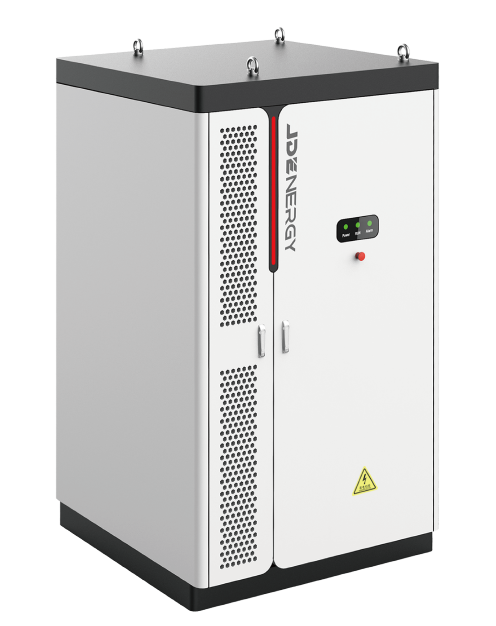
\includegraphics[width=12cm]{e-Block-250-Photo.png} \\[2cm]

    \vfill
    {\large\sffont Xi'an Singularity Energy Co., Ltd.}\\[0.5cm]
    {\color{gray} Version: V1.0 \quad | \quad Date: \today}
\end{titlepage}

% ==========================================
% Table of Contents
% ==========================================
\newpage
\pagenumbering{roman}
\tableofcontents
\newpage
\pagenumbering{arabic}

% ==========================================
% Chapter 1: About This Manual
% ==========================================
\section{About This Manual}
\subsection{Explanation of Symbols}
To ensure the safety of O\&M personnel and proper equipment operation, please familiarize yourself with the following symbols:

\vspace{1em}
\begin{tabularx}{\textwidth}{l l X}
\toprule
\textbf{Symbol} & \textbf{Name} & \textbf{Meaning for O\&M Safety} \\
\midrule

\includegraphics[height=1.2em]{warning.png} & {\sffont Warning} & Indicates content that, if not properly handled, may pose a danger to user safety or equipment. \\
\addlinespace

\includegraphics[height=1.2em]{attention.png} & {\sffont Attention} & Indicates content that may lead to equipment damage or performance degradation. \\
\addlinespace
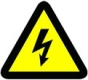
\includegraphics[height=1.2em]{electric.png} & {\sffont Electric} & Identifies parts with a risk of electric shock. \textbf{Do NOT touch} at will. \\
\addlinespace
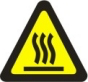
\includegraphics[height=1.2em]{temp.png} & {\sffont High Temp} & Identifies parts with high-temperature risks. \textbf{Do NOT touch} at will. \\
\addlinespace

\includegraphics[height=1.2em]{ground.png} & {\sffont Grounding} & Indicates the connection position for the protective earth (PE) wire. \\
\addlinespace
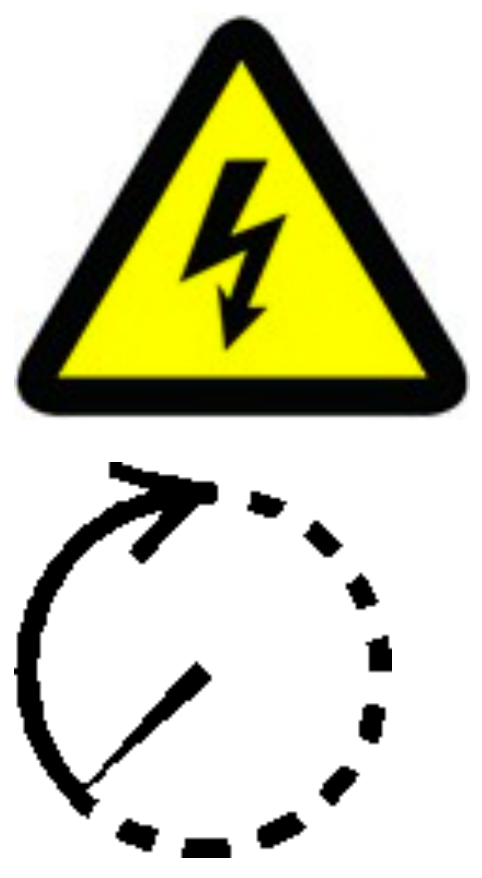
\includegraphics[height=1.2em]{cap_discharge.png} & {\sffont Discharge} & Operations by professionals only. Wait \textbf{30 minutes} after power-off before touching. \\
\bottomrule
\end{tabularx}
\vspace{1em}

\subsection{Scope of Application}
This manual is applicable to the routine O\&M of \textbf{eBlock-372/418 series}. It is intended for professional personnel with electrical expertise and experience in power distribution.

\subsection{Introduction to Energy Storage System}
The system consists of the \textbf{Intelligent Energy Block (eBlock)}, \textbf{Intelligent Energy Link (eLink)}, background monitoring, and transformers.

% ==========================================
% Chapter 2: Personnel Entry Safety Precautions
% ==========================================
\section{Personnel Entry Safety Precautions}
\begin{itemize}[leftmargin=1.5em]
    \item \textbf{Professional Qualification:} Only trained and qualified electrical technicians are allowed to operate the eBlock.
    \item \textbf{PPE Requirements:} Personnel must wear qualified protective equipment, including insulated gloves, shoes, and safety goggles.
    \item \textbf{Metal Objects:} Remove all metal objects (rings, watches, etc.) before operation.
    \item \textbf{Insulated Tools:} Use professional tools with insulated handles.
    \item \textbf{Capacitor Discharge:} Wait for at least \textbf{30 minutes} after power-off before touching any live components.
\end{itemize}

% ==========================================
% Chapter 3: On-site Operation Specifications
% ==========================================
\section{On-site Operation Specifications}
\subsection{Routine Inspection}
\begin{itemize}
    \item Check for water ingress, corrosion, or deformation of the cabinet.
    \item Monitor liquid cooling levels and pressure (standard static pressure: 0.8bar--1bar).
    \item Inspect cable connections for looseness or signs of overheating.
\end{itemize}

\subsection{Power On/Off Sequence}
\begin{itemize}
    \item \textbf{Power Off:} Disconnect the AC grid-side breaker first, then the DC-side breaker.
    \item \textbf{Power On:} Reverse the sequence; ensure system self-check is complete before closing.
\end{itemize}

% ==========================================
% Chapter 4: Abnormal Situation Handling Procedures
% ==========================================
\section{Abnormal Situation Handling Procedures}

\subsection{Fire Safety and Alarm Logic}
The system triggers tiered responses:
\begin{itemize}
    \item \textbf{Level 2 Alarm:} Smoke/CO/Temperature detected; the \textbf{Audible and Visual Alarm} activates.
    \item \textbf{Level 3 Alarm:} The system releases the fire extinguishing agent automatically.
\end{itemize}

\subsection{Emergency Response for Equipment Fire}
\begin{enumerate}
    \item \textbf{Power Isolation:} Immediately disconnect the power supply to the affected unit.
    \item \textbf{Evacuation:} Establish a cordon area with a radius of \textbf{100 meters}.
    \item \textbf{Initial Firefighting:} Use CO2 or dry powder extinguishers if safe to do so.
\end{enumerate}

\subsection{Other Abnormalities}
\begin{itemize}
    \item \textbf{Emergency Stop:} Press the red \textbf{Emergency Stop} button if there is an immediate threat.
    \item \textbf{Leakage/Odor:} Shut down immediately and contact technical support if unusual smells or leaks occur.
\end{itemize}

\end{document}
